\documentclass{sig-alt-release2}

\begin{document}
\conferenceinfo{PODC'09,} {August 10--12, 2009, Calgary, Alberta, Canada.} 
\CopyrightYear{2009}
\crdata{978-1-60558-396-9/09/08}
\title{Poster Abstract: PUSH, a Dataflow Shell}

\numberofauthors{2}
\author{
\alignauthor Noah Evans \\
\affaddr{Nara Institute of Science and Technology}\\
\affaddr{Nara, Japan}\\
\email{noah-e@is.naist.jp} 
\alignauthor Eric Van Hensbergen \\
\affaddr{IBM Research}\\
\affaddr{Austin, TX}\\
\email{bergevan@us.ibm.com}
}
\date{26 May 2009}

\maketitle

\begin{abstract}
This paper explores the use of extended shell pipeline operators to
establish distributed workflows and correlate results.
\end{abstract}

\vspace{1mm}
\noindent
{\bf Categories and Subject Descriptors:} C.2.4 {[Network Operating Systems]}: {Inferno}

\vspace{1mm}
\noindent
{\bf General Terms:} Design, Management 

\vspace{1mm}
\noindent
{\bf Keywords:} Supercomputing, Shell, Distributed Pipeline

High throughput computing is increasingly important in both scientific and business computing.

On the scientific side, massive data provided by telescopes, biological, molecular and other databases 

on the business side,  sensor networks, 
online transactions, video transcoding and distribution among many other examples provide huge amounts of data to process. 

You end up making huge networks of processes and then manually batching, stichting these processes together. The supercomputer realm is still maintaing batch style processes, the business world has dataflow tools which simplify the construction of these webs of dataflow processes. but each system provides its own interface. 


However there are still no clear, portable ways to create and instantiating these. There are a lot of different systems, Hadoop, Dryad, Streamit but they all provide graphical interfaces(Dryad), program language integration(DryadLINQ). There is no clear general way of handling things like the unix shell. (note that some projects have syntax similar to the unix shell, but they are *not* shells).  Each has their own instantiating the processes. Moreover they are implemented as middleware. 

In this short paper we present Push, a shell which takes traditional unix style pipeline utilities and creates arbitrary dataflow graphs using a shell. With Push the user can make create arbitrary graphs of pipelines using "fanout" and "fanin" operators which allow processes to create sets of one to many and many to one pipelines. The composition of these pipelines are designed by the shell but the pipelines themselves are entirely implemented by the underlying system. By trusting the underlying system to take the created process graphs, instantiate . Push provides a general, portable and simple interface that takes traditional unix pipeline executables and incorporates these programs, already designed from traditional pipelines, and allows them to work in a data flow model. Push is intended to be used with a process running . Push was specifically designed to work with the Unified Execution Model(UEM)\cite{} in order to 


As super computers get larger and applications move into the cloud, coming up with simple 
As part of the HARE project[cat] one of the central problems of using a huge system like that is that there really isn't good ways to get processes running and executed. Specifying tasks is aso very difficult. . and attempting to build this also boils 

Right now individual processes are assigned to lightweight kernels and then the machine is rebooting leading to switches between processes that take more than one minute \cite{colorad}

Right now there is progress. 

We also observe that much of the cloud computing world has many of the same problems. 

creating batch processes that try to boot things. 

These force recompiling, rebooting or choosing a complete operating system to boot. 

These problems, rebooting and marshaling of batch jobs are similar to the problems occuring with cloud systems, epitomized by Amazon's EC2. While cloud systems offer growing pools of compute value, booting systems and migration of operating systems mean that cloud systems have many of the same problems. 

we feel that in both of these systems this is a shame because they go away from the unix way, which provided. 

That both supercomputer and cloud systems are having the same problems. Trying to run batch jobs, where huge amounts are. 

One of the central advantages of unix was that it created a standard way of dealing with a huge time sharing system interactively. 

\section{Challenges}

The HARE project attempts to address the complexity of super computer settings by providing a right weight kernel that provides much of the advantages of a light weight kernel(speed, data throughput) with a heavyweight kernel(the ability to run multiple processes, scheduling, separation between kernel and user processes). 

creating a single system image. how do you fork?  

the unix pipeline model does not work so well when you are potentially over a network or you have limited memory bandwidth. The goal is to minimize memory copying. 



However the having a kernel that provides a nice medium between kernel types is not useful unless there is a 

How do you create a uniform execution model this. 

However a uniform execution is not useful without something to run on it. 

Right now there are ad hoc batch schedulers that can dispatch and run different machines. However there are no systems that provide a uniform view of the entire system and run processes on them in a transparent way like the unix shell. 

However the problem comes from creating huge sets of arbitrary pipelines. 


a standard, system agnostic syntax for running unix executables using composable streams. 

goal is a clear syntax that expresses data flow operations while at the same time being a general solution. unix shells work the same as long as their system calls are consistent. Push supports both the usual system calls of unix(read, write, fork, dup) as well as a new scalable based on UEM. 

treat the act of composing, creating and writing to and from pipelines as a system level problem. Push makes no assumptions regarding this. 

By pushing these discussions to the operating system. 

Push builds 

push has a separate file for dealing with forking. general local aspects of the system are dealt 

\seciton{Push}

Push is based. 


We are interested 

While this is usua

We are running 

Distributed data flow systems, 
In typical DISC systems, 
runtimes~\cite{dean2008msd}~\cite{bialecki:hfr}~\cite{isard2007ddd} define 
graphs of processes, the edges of the graphs representing 
pipes and their vertices represent computation on a system.  
Within these runtimes a new class of 
languages~\cite{pike2005idp}~\cite{yu2008dsg}~\cite{olston2008pln} can be used by researchers to solve "pleasantly parallel" 
problems more quickly without worrying about explicit concurrency.

These languages provide automated control flow(typically matched to the 
architecture of the underlying runtime) and channels of communication between 
systems.
In existing systems, these workflows and the underlying computation are 
tightly linked, tying solutions to a particular runtime, workflow and language.
This creates difficulties for analytics researchers who wish to draw upon
tools written in many different languages or runtimes which may be available
on several different architectures or operating systems.

We observe that UNIX pipes were designed to get around 
many of these incompatibilities, allowing developers to hook together tools 
written in different languages and runtimes in ad-hoc fashions.  
This allowed tool developers to focus on doing one thing well, and
enabled code portability and reuse in ways not originally conceived by
the tool authors.  The UNIX shell incorporated a model for tersely composing 
these smaller tools in pipelines (e.g. 'sort $|$ uniq -c'),  
creating coherent workflow to solve more complicated problems 
quickly. 
Tools read from standard input and wrote to standard output, allowing programs 
to work together in streams \emph{with no explicit knowledge of this chaining
built into the program itself}.

One to one pipelines such as those used by a typical UNIX shell, can not be 
trivially mapped to DISC workflows which incorporate one-to-many, many-to-many,
and many-to-one data flows. 
Additionally, typical UNIX pipeline tools write data according to buffer 
boundaries instead of record boundaries.
As \cite{pike2005idp} notes DISC systems need to be able to cleanly separate 
input streams into records and then show that the order of these records is 
independent. 
By separating input and output into discrete unordered records data can be 
easily distributed and coalesced.

To address these issues we have implemented a prototype shell, 
which we call PUSH, using DISC principles and incorporating extended 
pipeline operators to establish distributed workflows and correlate results.
Our implementation is based on extending an existing shell, MASH, 
from which we inherited a rich interpreted scripting language. 
It treats variables as lists of strings and has no native handling for any 
other data type. 
Integer expression handling and other facilities are provided by shell commands. 
It has native regular expression support and it has a novel ability to do 
declarative shell programming through a make like syntax incorporated in the 
shell itself.

\begin{figure}[htp]
\centering
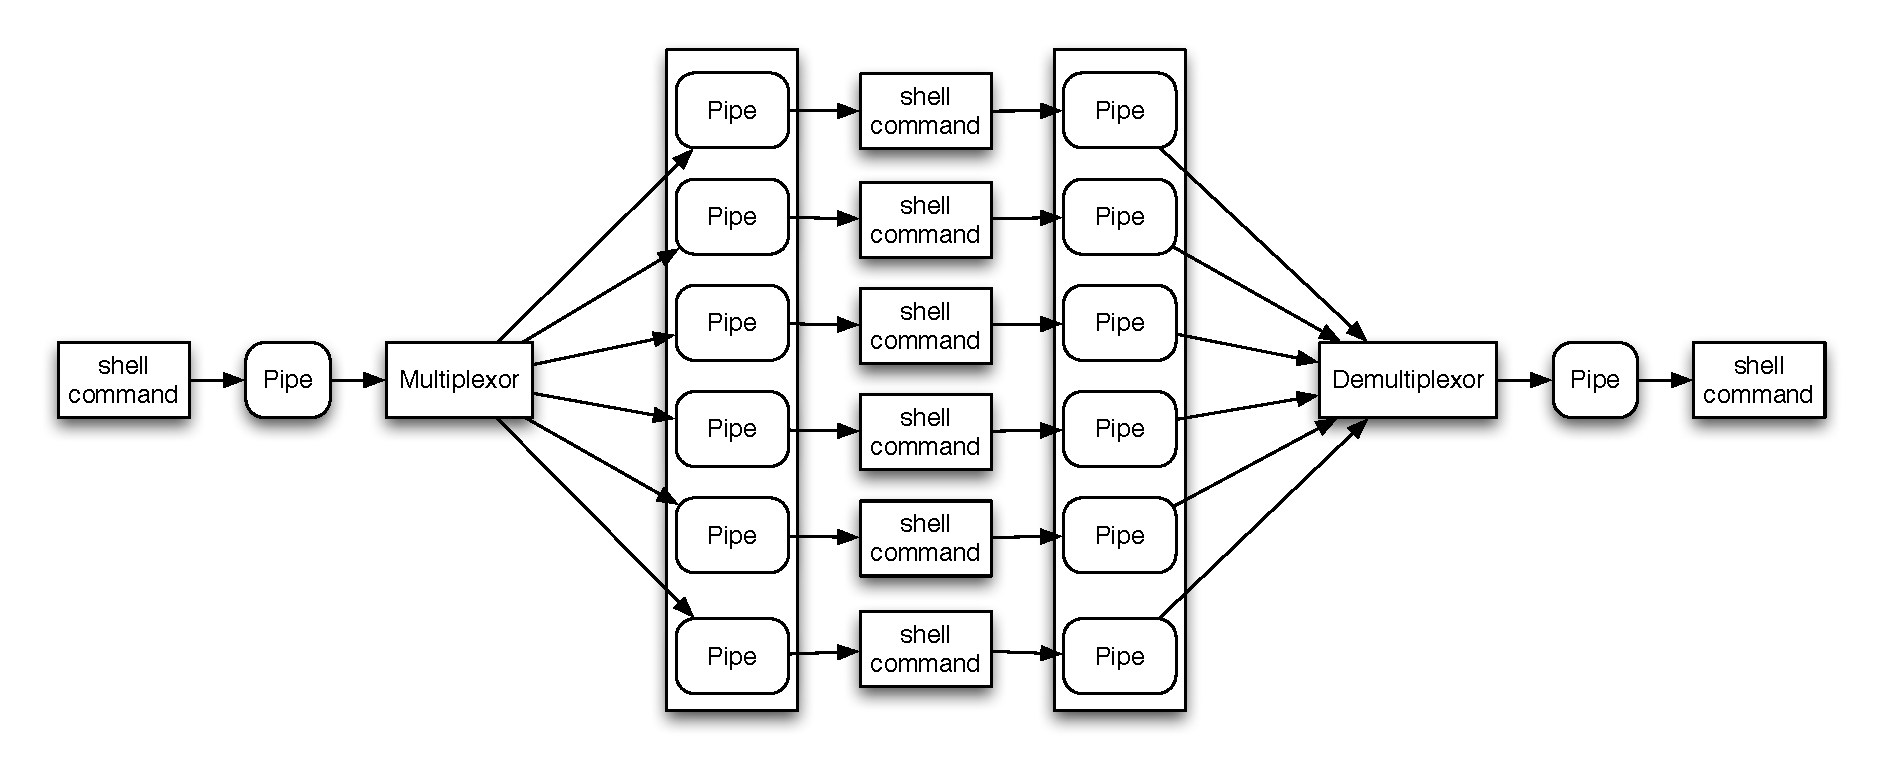
\includegraphics[width=3in]{pipestruct.eps}
\caption{The structure of the PUSH shell}
\label{fig:pipestruct} 
\end{figure}

We have added two additional pipeline operators, 
a multiplexing fan-out(\verb!|<![\emph{n}]), and a coalescing fan-in(\verb!>|!). 
This combination allows PUSH to distribute I/O to and from multiple
simultaneous threads of control.
The fan-out argument \emph{n} specifies the desired degree of parallel 
threading.  If no argument is specified, the default of spawning a new
thread per record (up to the limit of available cores) is used.  This can
also be overriden by command line options or environment variables.
The pipeline operators provide implicit grouping semantics allowing natural 
nesting and composibility.
While their complimentary nature usually lead to symmetric
mappings (where the number of fan-outs equal the number of fan-ins), there is 
nothing within our implementation which enforces it.
Normal redirections as well as application specific sources and sinks 
can provide alternate data paths.
Remote thread distribution and interconnect are composed and managed
using synthetic file systems in much the same manner as Xcpu, 
pushing the distributed complexity into the middleware in an language and 
runtime neutral fashion.

PUSH also differs from traditional shells by implementing native support for 
record based input handling over pipelines. This facility is similar to the 
argument field separators, IFS and OFS, in traditional shells which use a 
pattern to determine how to tokenize arguments. PUSH provides two variables, 
ORS and IRS, which point to record separator modules. These modules 
(called multiplexors in PUSH) split data on record boundaries, emitting 
individual records that the system distributes and coalesces. 

The choice of which multipipe to target is left as a decision to the module. 
Different data formats may have different output requirements. 
Demultiplexing from a multipipe is performed by creating a many to one 
communications channel within the shell. The shell creates a reader processes 
which connects to each pipe in the multipipe. When the data reaches an 
appropriate record boundary a buffer is passed from the reader to the shell 
which then writes each record buffer to the output pipeline. 

An example from our particular experience, Natural Language Processing, is 
to apply an analyzer to a large set of files, a "corpus". User programs go 
through each file which contain a list of sentences, one sentence per line. 
They then tokenize the sentence into words, finding the part of speech and 
morphology of the words that make up the sentence.
This sort of task maps very well to the DISC model. There are a large number of 
discrete sets of data whose order is not necessarily important. We need to 
perform a computationally intensive task on each of the sentences, which are 
small, discrete records and ideal target for parallelization. 

PUSH was designed to exploit this mapping. For example, to get a histogram of 
the distribution of Japanese words from a set of documents using chasen, 
a Japanese morphological analyzer, we take a set of files containing sentences 
and then distribute them to a cluster of machines on our network. The command 
is as follows:

\begin{verbatim}
push -c '{
  ORS=./blm.dis
  du -an files |< xargs os \\
   chasen | awk '{print \$1}' | sort | uniq -c \\
   >| sort -rn
}'
\end{verbatim}

The first variable, ORS, declares our record multiplexor module, the intermediary 
used to ensure that the input and output to distributed pipes are correctly 
aligned to record boundaries. du -n gives a list of the files (note that our 
du is a bit different from the canonical UNIX du, it replaces much of find's 
functionality) which are then "fanned out"(\verb!|<!) using a combination 
of a \emph{multipipe}, an ordered set of pipes, and a \emph{multiplexor} 
which determines which pipes are the targets of each unit of output.  
This fanned out data goes to xargs on other machines which 
then uses the filenames(sent from the instantiating machine) as arguments to 
chasen. The du acts as a command driver, fanning out file names to the 
individual worker machines. The workers then use the filenames input to 
xargs, which uses the input filenames as arguments to xargs target command. 
Using the output of the analyzer awk extracts the first line fields(Japanese 
words) which are then sorted and counted using uniq.  Finally these word 
counts are "fanned in"(\verb!>|!) to the originating machine which then 
sorts them. 

% status and future work


Because PUSH distributes streaming data over potentially remote links push 
is prone to causing network congestion between nodes. 
We are investigating multiple approaches to mitigating this overhead, both
by using parallel distributed file systems and/or using distributed
databases such as Google's Bigtable.
One research challenge is to find a way to integrate reference to these
external data resources (or record sets within these resources) with the
distributed pipelines in a natural fashion.

Another area of ongoing exploration is looking at adding fault tolerance as 
well as a more automated mechanism for determining how many resources to 
allocate to a particular problem and automatically adapting that provisioning 
based on monitoring the changing workload as it executes on the 
cluster.

PUSH is under active development, but the current source code is open source 
and available on Google Code.
This work has been supported by the Department of Energy Of Office of Science Operating and Runtime Systems for Extreme Scale Scientific Computation project under contract \#DE-FG02-08ER25851. 


\bibliographystyle{plain}

\begin{thebibliography}{1}

\bibitem{bialecki:hfr}
A.~Bialecki, M.~Cafarella, D.~Cutting, and O.~O~Malley.
\newblock {Hadoop: a framework for running applications on large clusters built
  of commodity hardware, 2005}.
\newblock {\em Wiki at http://lucene. apache. org/hadoop}.

\bibitem{bryant2007dis}
R.E. Bryant.
\newblock {Data-Intensive Supercomputing: The case for DISC}.
\newblock Technical report, Tech Report CMU-CS-07-128, Carnegie Mellon
  University, School of Computer Science, 2007.

\bibitem{dean2008msd}
J.~Dean and S.~Ghemawat.
\newblock {MapReduce: Simplified Data Processing on Large Clusters}.
\newblock {\em Communications of the ACM}, 51(01):7, 2008.

\bibitem{isard2007ddd}
M.~Isard, M.~Budiu, Y.~Yu, A.~Birrell, and D.~Fetterly.
\newblock {Dryad: distributed data-parallel programs from sequential building
  blocks}.
\newblock In {\em Proceedings of the 2007 conference on EuroSys}, pages 59--72.
  ACM Press New York, NY, USA, 2007.

\bibitem{olston2008pln}
C.~Olston, B.~Reed, U.~Srivastava, R.~Kumar, and A.~Tomkins.
\newblock {Pig latin: a not-so-foreign language for data processing}.
\newblock In {\em Proceedings of the 2008 ACM SIGMOD international conference
  on Management of data}, pages 1099--1110. ACM New York, NY, USA, 2008.

\bibitem{pike2005idp}
R.~Pike.
\newblock {Interpreting the data: Parallel analysis with Sawzall}.
\newblock {\em Scientific Programming}, 13(4):277--298, 2005.

\bibitem{yu2008dsg}
Y.~Yu, M.~Isard, D.~Fetterly, M.~Budiu, U.~Erlingsson, P.K. Gunda, and
  J.~Currey.
\newblock {DryadLINQ: A system for general-purpose distributed data-parallel
  computing using a high-level language}.
\newblock In {\em Symposium on Operating System Design and Implementation
  (OSDI), San Diego, CA, December}, pages 8--10, 2008.

\end{thebibliography}
\end{document}
